\section{Protocolos de roteamento em redes \textit{ad hoc}}\label{protocols}

Em redes m\'oveis \textit{ad hoc}, uma rota entre dois n\'os pode ser formada por saltos atrav\'es de um ou mais n\'os na rede, na qual, cada salto representa uma passagem por diferentes n\'os at\'e chegar ao destino desejado. 

Os protocolos de roteamento em redes \textit{ad hoc} precisam trabalhar, constantemente, com as trocas de topologia da rede, a qual acarreta em atualizar ou procurar novas rotas entre os n\'os da rede. 
A troca de topologia ocorre quando um n\'o da rede se desloca fisicamente na \'area de comunica\c{c}\~ao, alterando a conex\~ao com os vizinhos, e encontra novas ou perde antigas conex\~oes.

Os protocolos de roteamento s\~ao variados, mas segundo \cite{gorantala}, somente dois s\~ao de suma import\^ancia nas redes \textit{ad hoc}, sendo o DSDV(\textit{Destination Sequenced Distance Vector}), para redes pequenas, e o AODV(\textit{Ad-hoc On-Demand Distance Vector}), para redes \textit{ad hoc} em geral. 
Cada protocolo trabalha de forma diferente, podendo ser pr\'o-ativo ou reativo. 
"Os protocolos pr\'o-ativos mant\^em rotas para todos os n\'os da rede, independente do uso ou necessidade destas rotas. (...) J\'a os protocolos reativos iniciam as atividades de roteamento de acordo com a demanda" \cite{pereira}.

Os protocolos de roteamento estudados s\~ao baseados em dois tipos de algoritmos, em Vetor de Dist\^ancia, ou em Estado de Enlace. 
Os protocolos baseados em Vetor de Dist\^ancia possuem as tabelas de roteamento atualizadas atrav\'es da troca de mensagens com seus vizinhos, e mant\'em apenas as melhores rotas nesta tabela. 
Em intervalos de tempos regulares, as tabelas de roteamento s\~ao enviadas apenas para seus vizinhos, que por sua vez, atualizam suas tabelas. 
E o protocolo de roteamento que \'e baseado em Estado de Enlace tamb\'em possui as tabelas de roteamento atualizadas atrav\'es da troca de mensagens com seus vizinhos, por\'em, mant\'em todas as informa\c{c}\~oes de conex\~oes da rede na tabela. 
O pr\'oprio protocolo descobre o melhor caminho, pois a rota possui o identificador de interface, n\'umero de enlace e m\'etrica. 
No momento em que ocorre uma altera\c{c}\~ao no estado de enlace da rede, os n\'os adjacentes percebem e notificam os vizinhos, que por sua vez, atualizam a rota se ela for nova \cite{posselt}.

Os roteadores em uma rede \textit{ad hoc} trocam informa\c{c}\~oes de roteamento uns com os outros, com a finalidade de tomar conhecimento das disponibilidades de rotas e da topologia da rede \cite{pereira}. 
Essa troca de informa\c{c}\~oes pode acarretar em \textit{loop} de roteamento, o qual \'e uma condi\c{c}\~ao em que um pacote \'e transmitido continuamente em uma s\'erie de n\'os, sem sequer alcan\c{c}ar seu n\'o de destino desejado. 
Esse \textit{loop} pode ocorrer quando dois ou mais n\'os t\^em informa\c{c}\~oes de roteamento que indicam, de forma incorreta, que uma rota \'e v\'alida para um n\'o de destino. Por\'em, esse n\'o de destino \'e inalcan\c{c}\'avel atrav\'es desta mesma rota. 
Essa \'e mais uma condi\c{c}\~ao em que os protocolos de roteamento precisam trabalhar e corrigir \cite{hengartnet}.

As subse\c{c}\~oes \ref{subDSDV}, \ref{subAODV} e \ref{subOLSR} apresentam os protocolos DSDV, AODV e OLSR, respectivamente, os quais s\~ao analisados nos experimentos desse trabalho.

\subsection{\textit{Destination sequenced distance vector} - DSDV}\label{subDSDV} 
O protocolo DSDV \'e um protocolo de roteamento pr\'o-ativo\cite{gorantala}, baseado no algoritmo de vetor de dist\^ancias, que trabalha requisitando periodicamente, de cada um dos n\'os vizinhos, suas tabelas de roteamento, com a finalidade de mant\^e-las atualizadas. 
Cada n\'o da rede mant\'em uma tabela de roteamento, contendo o pr\'oximo salto e o n\'umero de saltos para cada destino alcan\c{c}\'avel. 
As tabelas incluem rotas para todos os n\'os da rede, mesmo que nunca seja necess\'ario enviar pacote para este n\'o. 
Cada n\'o mant\'em apenas uma rota para cada destino.

Os \textit{loops} de rotas podem ocorrer quando informa\c{c}\~oes de roteamento incorretas s\~ao mantidas na rede ap\'os uma troca de topologia. 
Geralmente, ocorre quando um n\'o detecta uma queda no enlace com o n\'o vizinho e, antes que consiga propagar sua nova tabela, recebe de outro n\'o informa\c{c}\~ao desatualizada referente \`a conex\~ao interrompida. 
A vantagem principal do DSDV sobre os protocolos baseados em Vetor de Dist\^ancias tradicionais \'e que ele garante a aus\^encia de \textit{loops}, usando o conceito de n\'umero de sequ\^encia mantido em cada rota. 
O n\'umero de sequ\^encia \'e estabelecido pelo n\'o destino e \'e incrementado a cada novo aviso de rota.
As rotas mais recentes possuem um n\'umero de sequ\^encia maior e s\~ao as mais favor\'aveis. 
Caso os n\'umeros de sequ\^encia sejam iguais, a rota que tiver o menor n\'umero de saltos ser\'a a mais favor\'avel. 
Neste contexto, o uso de n\'umeros de sequ\^encia faz com que o DSDV se adapte melhor para redes de topologia din\^amica como redes \textit{ad hoc}.

\subsubsection{Exemplo de funcionamento do DSDV}

A Figura \ref{figOpDSDV}, descreve uma rede com 8 hosts. 
Pode-se analisar a mudan\c{c}a de roteamento da tabela do MH4 em rela\c{c}\~ao ao movimento do \textit{host} MH1(\textit{Mobile Host} 1), onde o movimento \'e representado pelas setas com estilo pontilhado. 

\begin{figure}[H]
	\centering
	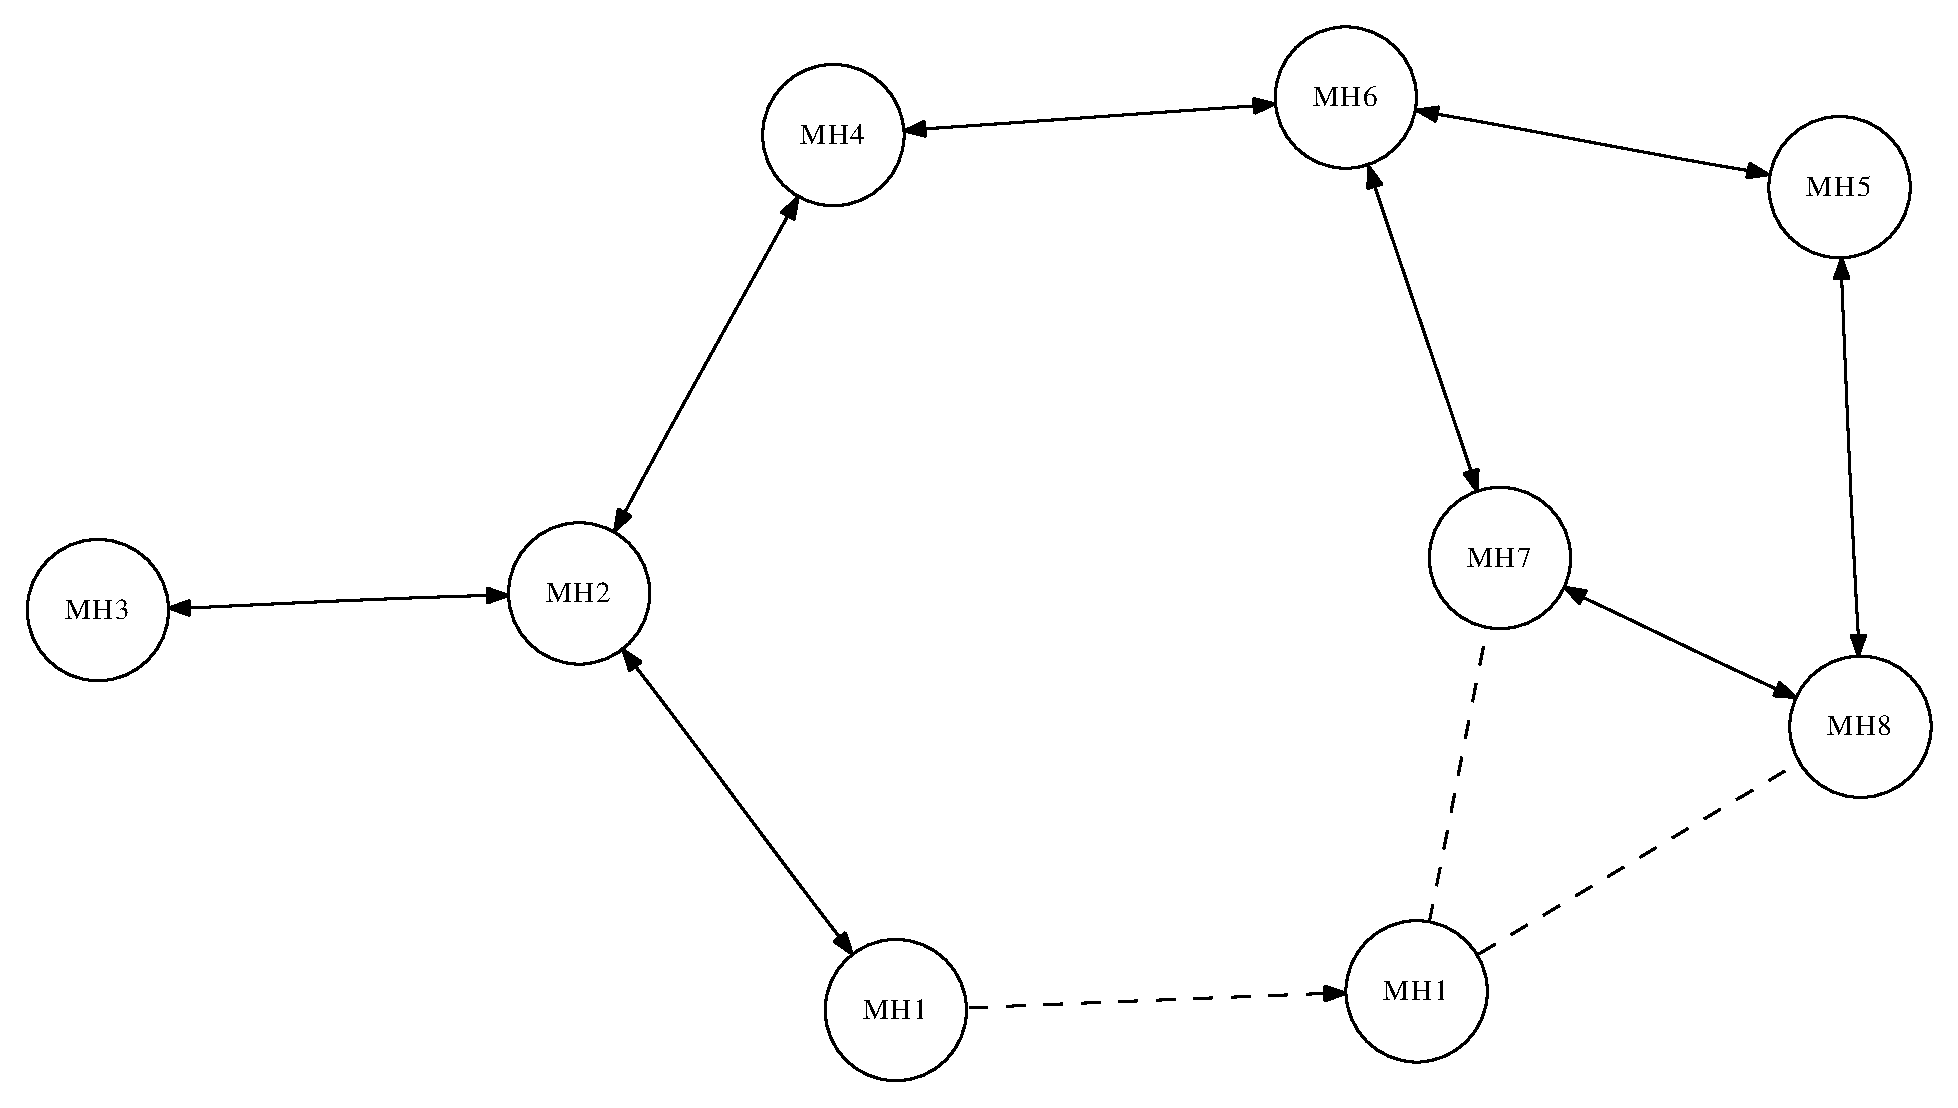
\includegraphics[scale=.4]{dsdvOperation.eps}
	\caption{Exemplo de opera\c{c}\~ ao do DSDV}
	\label{figOpDSDV}
\end{figure}

Uma tabela de roteamento do DSDV, cont\'em, para cada n\'o na rede:
\begin{itemize}
	\item Informa\c{c}\~oes do n\'o de destino;
	\item o pr\'oximo salto na rota para alcan\c{c}ar o destino;
	\item a m\'etrica com o valor de quantos saltos s\~ao necess\'arios para alcan\c{c}ar o destino;
	\item o n\'umero de sequ\^encia utilizado para sincroniza\c{c}\~ao das rotas;
	\item o install, atuando como um marcador de tempo da rota, para decidir de deletar ou n\~ao uma nova informa\c{c}\~ao topol\'ogica; e
	\item o campo informa\c{c}\~ao, servindo como um ponteiro para indicar a tabela com informa\c{c}\~oes sobre a estabilidade da rota.
\end{itemize}

Inicialmente, todos os n\'os anunciam suas informa\c{c}\~oes de roteamento para todos os outros n\'os da rede e, portanto, a tabela de roteamento do \textit{host} MH4 inicialmente apresenta o seguinte conte\'udo conforme a Tabela \ref{tabRtMH4}.

\begin{table}[H]
	\centering
	\caption{Tabela de roteamento do \textit{host} MH4 \cite{pebha}}
	\begin{tabular}{ | c | c | c | c | c | c | }
		\hline
		Destino & Pr\'oximo salto & M\'etrica & N\'umero de sequ\^encia & Install & Informa\c{c}\~ao \\ \hline
		MH1 & MH2 & 2 & S406\_MH1 & T001\_MH4 & Ptr1\_MH1 \\ \hline
		MH2 & MH2 & 1 & S128\_MH2 & T001\_MH4 & Ptr1\_MH2 \\ \hline
		MH3 & MH2 & 2 & S564\_MH3 & T001\_MH4 & Ptr1\_MH3 \\ \hline
		MH4 & MH4 & 0 & S710\_MH4 & T001\_MH4 & Ptr1\_MH4 \\ \hline
		MH5 & MH6 & 2 & S309\_MH5 & T002\_MH4 & Ptr1\_MH5 \\ \hline
		MH6 & MH6 & 1 & S076\_MH6 & T001\_MH4 & Ptr1\_MH6 \\ \hline
		MH7 & MH6 & 2 & S128\_MH7 & T002\_MH4 & Ptr1\_MH7 \\ \hline
		MH8 & MH6 & 3 & S050\_MH8 & T002\_MH4 & Ptr1\_MH8 \\ \hline
	\end{tabular}
	\label{tabRtMH4}
\end{table}

Por\'em, quando o \textit{host} MH1 move sua localiza\c{c}\~ao para pr\'oximo dos \textit{hosts} MH7 e MH8 como apresentado na Figura \ref{figOpDSDV} ent\~ao, o enlace entre MH2 e MH1 vai ser quebrado.
Isto resulta em atribui\c{c}\~ao de uma m\'etrica infinita de MH2 para MH1 e o n\'umero de sequ\^encia ser\'a alterado para um n\'umero \'impar na tabela de roteamento em MH2, que atualizar\'a essa informa\c{c}\~ao para os \textit{hosts} vizinhos. 
Desde que haja um novo \textit{host} vizinho para MH7 e MH8, eles v\~ao atualizar essa informa\c{c}\~ao nas respectivas tabelas de roteamento e propagar essa nova informa\c{c}\~ao. 
Agora, MH4 receber\'a esta atualiza\c{c}\~ao de informa\c{c}\~ao de MH6, onde MH6 recebe 2 pacotes de informa\c{c}\~oes de diferentes vizinhos para chegar em MH1 com o mesmo n\'umero de sequ\^encia, mas com diferentes m\'etricas. 
A sele\c{c}\~ao da rota ir\'a depender da menor contagem de saltos quando o n\'umero de sequ\^encia \'e o mesmo. 
A tabela de roteamento do MH4 estar\'a com o conte\'udo demonstrado na Tabela  \ref{tabNewRtMH4}.

\begin{table}[H]
	\centering
	\caption{Tabela de roteamento do \textit{host} MH4 depois do movimento do \textit{host} MH1 \cite{pebha}}
	\begin{tabular}{ | c | c | c | c | c | c | }
		\hline
		Destino & Pr\'oximo salto & M\'etrica & N\'umero de sequ\^encia & Install & Informa\c{c}\~ao \\ \hline
		MH1 & MH6 & 3 & S516\_MH1 & T001\_MH4 & Ptr1\_MH1 \\ \hline
		MH2 & MH2 & 1 & S238\_MH2 & T001\_MH4 & Ptr1\_MH2 \\ \hline
		MH3 & MH2 & 2 & S674\_MH3 & T001\_MH4 & Ptr1\_MH3 \\ \hline
		MH4 & MH4 & 0 & S820\_MH4 & T001\_MH4 & Ptr1\_MH4 \\ \hline
		MH5 & MH6 & 2 & S502\_MH5 & T002\_MH4 & Ptr1\_MH5 \\ \hline
		MH6 & MH6 & 1 & S186\_MH6 & T001\_MH4 & Ptr1\_MH6 \\ \hline
		MH7 & MH6 & 2 & S238\_MH7 & T002\_MH4 & Ptr1\_MH7 \\ \hline
		MH8 & MH6 & 3 & S160\_MH8 & T002\_MH4 & Ptr1\_MH8 \\ \hline
	\end{tabular}
	\label{tabNewRtMH4}
\end{table}

\subsubsection{Vantagens do DSDV}
\begin{itemize}
	\item Livre de \textit{loops} \cite{gorantala}.
	\item Problemas com contagem ao infinito \'e reduzido no DSDV \cite{gorantala}.
	\item Pode-se evitar tr\'afego extra com atualiza\c{c}\~oes incrementais, em vez de atualiza\c{c}\~oes de despejo completo.
	\item Sele\c{c}\~ao de caminho: O DSDV mant\'em somente o melhor caminho em vez de manter v\'arios caminhos para um mesmo destino. Com isso, o espa\c{c}o da tabela de roteamento \'e reduzido.
\end{itemize}

\subsubsection{Limita\c{c}\~ oes do DSDV}
\begin{itemize}
	\item Desperd\'icio do uso da banda na rede devido \`a propaga\c{c}\~ao desnecess\'aria de informa\c{c}\~oes de roteamento, mesmo se n\~ao houver mudan\c{c}as na topologia da rede \cite{Patel00energyin}.	
	\item O DSDV n\~ao suporta m\'ultiplos caminhos de rotas \cite{gorantala}.
	\item \'E dif\'icil determinar um tempo de converg\^encia para a propaga\c{c}\~ao das rotas \cite{heg}.
	\item \'E dif\'icil manter a propaga\c{c}\~ao das tabelas de rotas para uma grande rede. Cada \textit{host} na rede deve manter uma tabela de rotas para propaga\c{c}\~ao. Mas para uma grande rede, isso causaria \textit{overhead} de rede, o qual consome uma maior banda na rede \cite{gorantala}.
\end{itemize}
	%Destination sequenced distance vector - DSDV
\subsection{\textit{Ad hoc on demand distance vector} - AODV}
O protocolo AODV \'e um protocolo reativo, baseado em vetor de dist\^ancias, e pode ser considerado como uma combina\c{c}\~ao de outros dois protocolos, denominados DSR e DSDV. 
O AODV tem a base do DSR, o qual \'e baseado sob demanda, ou seja, descobre rotas somente quando necess\'ario, e utiliza os mecanismos de descoberta de rotas e manuten\c{c}\~ao de rotas.
Entretando, o AODV utiliza a caracter\'istica do DSDV de obrigar todos os n\'os intermedi\'arios a estabelecerem dinamicamente entradas em tabelas de roteamento locais para cada destino ativo.
Cada n\'o tem conhecimento do pr\'oximo salto para alcan\c{c}ar o destino e a dist\^ancia em n\'umero de saltos.
Pode ser considerado como uma vers\~ao melhorada do DSDV, uma ver que seu funcionamento baseado em demanda minimiza o n\'umero de inunda\c{c}\~oes na rede exigido pelo DSDV para cria\c{c}\~ao de rotas.

\subsubsection{Limita\c{c}\~oes e desvantagens do AODV}
\begin{description}
	\item[Necessidade de um meio de propaga\c{c}\~ ao:] O algoritmo necessita que os n\'os no meio da propaga\c{c}\~ ao possam detectar outros 
	\item[N\~ao reutiliza informa\c{c}\~oes de roteamento] O AODV carede de efici\^encia na t\'ecnica de manuten\c{c}\~ao de suas rotas. Informa\c{c}\~oes de roteamento s\~ao sempre atualizadas em cada demanda, inclu\'indo casos comuns de tr\'afego. \cite{ramachandran}
\end{description}
	%Ad hoc on demand distance vector} - AODV
\subsection{\textit{Optimized link state routing} - OLSR}
O protocolo OLSR \cite{rfc3626} \'e um protocolo pr\'o-ativo, baseado em estado de conex\~ao, onde cada n\'o possui as informa\c{c}\~oes de rotas e compartilham entre si constantemente. 
O diferencial desse protocolo em rela\c{c}\~ao ao DSDV, que tamb\'em \'e pro-\'ativo, por\'em baseado em dist\^ancia de vetores, \'e que o OLSR diminui o tr\'afego de informa\c{c}\~oes de roteamento utilizando somente alguns n\'os pr\'e-selecionados, para retransmitir as mensagens de descoberta de rotas na rede.
Essa t\'ecnica \'e denominada MPR (\textit{Multipoint Relay}).

\subsubsection{Exemplo de funcionamento do OLSR}
Considerando as Figuras \ref{fig:olsrComum} e \ref{fig:olsrOperation}, temos a diferen\c{c}a de funcionamento de descoberta de rotas a cada passo, onde cada n\'o repassa as informa\c{c}\~oes de rotas entre os n\'os vizinhos.

\begin{figure}[H]
	\centering
	\subfigure[Primeiro est\'agio]{
		\includegraphics[scale=0.3]{olsrOperationStep1.eps}
	}\label{subfig:olsrStep11}
	\subfigure[Segundo est\'agio]{
		\includegraphics[scale=0.3]{olsrOperationStep2.eps}
	}\label{subfig:olsrStep12}
	\subfigure[Terceiro est\'agio]{
		\includegraphics[scale=0.3]{olsrOperationStep3.eps}
	}\label{subfig:olsrStep13}
	\subfigure[Quarto est\'agio]{
		\includegraphics[scale=0.3]{olsrOperationStep4.eps}
	}\label{subfig:olsrStep14}	
	\caption{Descoberta de rotas do protocolo DSDV}
	\label{fig:olsrComum}
\end{figure}

O mecanismo para selecionar os vizinhos que ir\~ao retransmitir os pacotes, denominado MPR, \'e simples. Ele escolhe vizinhos alcan\c{c}\'aveis atrav\'es de um salto que tenham comunica\c{c}\~ao sim\'etrica, bidirecional, com pacotes de mensagens \textit{HELLO}

\begin{figure}[H]
	\centering
	\subfigure[Primeiro est\'agio]{
		\includegraphics[scale=0.3]{olsrOperationStep1.eps}
	}\label{subfig:olsrStep21}
	\subfigure[Segundo est\'agio]{
		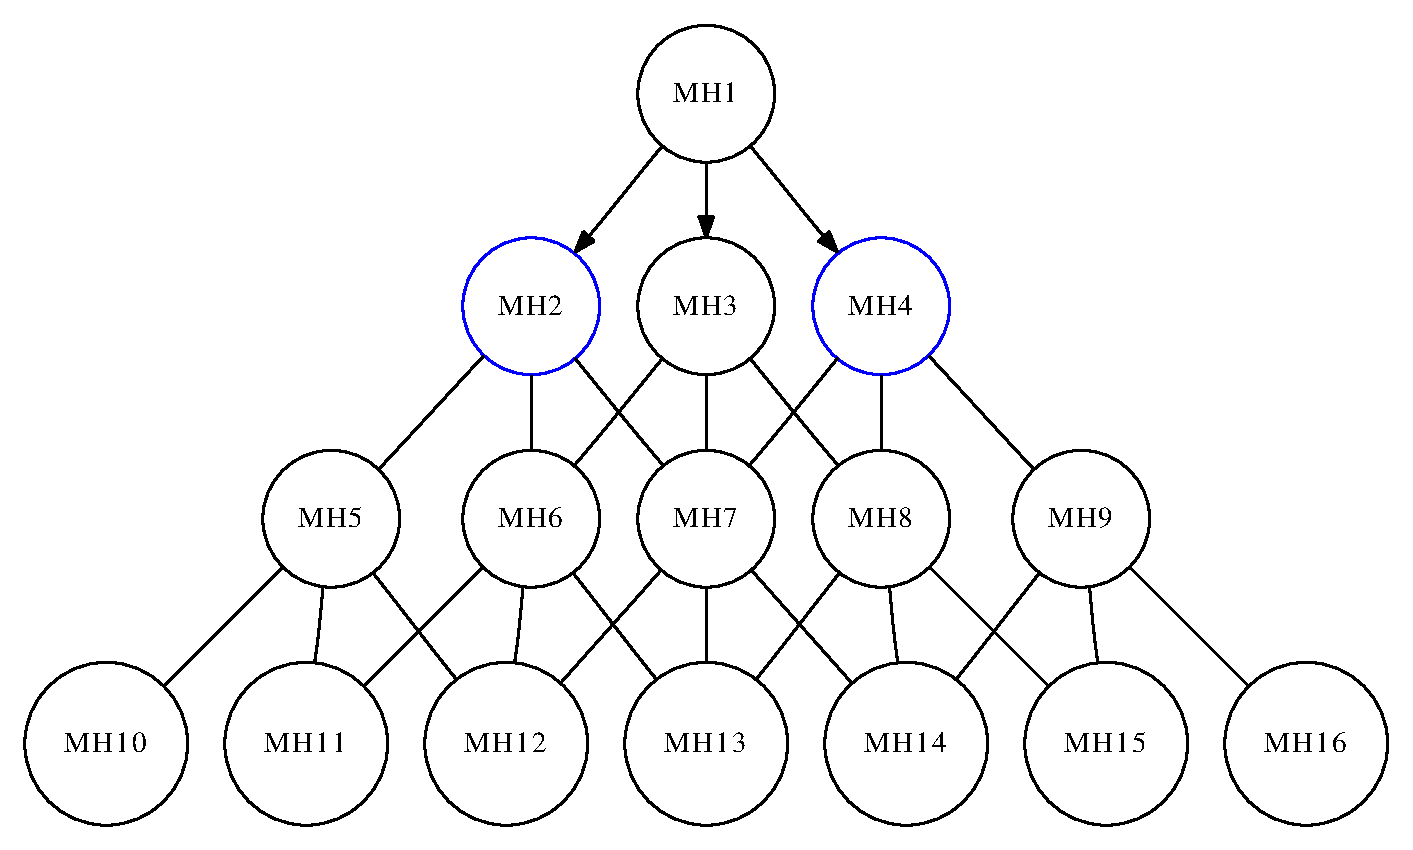
\includegraphics[scale=0.3]{olsrOperationStep5.eps}
	}\label{subfig:olsrStep22}
	\subfigure[Terceiro est\'agio]{
		\includegraphics[scale=0.3]{olsrOperationStep6.eps}
	}\label{subfig:olsrStep23}
	\subfigure[Quarto est\'agio]{
		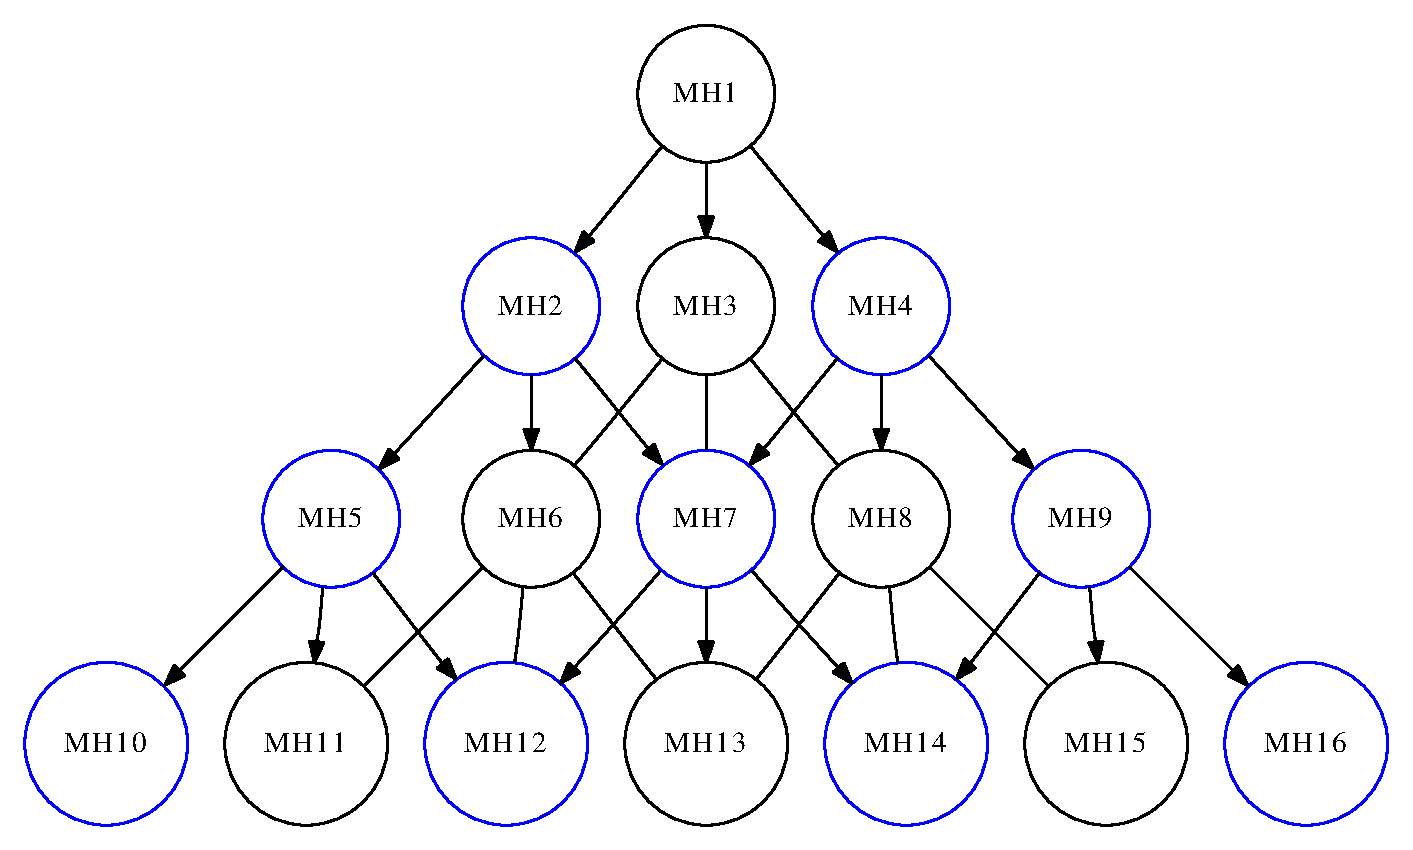
\includegraphics[scale=0.3]{olsrOperationStep7.eps}
	}\label{subfig:olsrStep24}	
	\caption{Descoberta de rotas do protocolo OLSR}
	\label{fig:olsrOperation}
\end{figure}


	%Optimized link state routing - OLSR
\subsection{Comparativo entre os protocolos} 
A tabela \ref{tabCompProt} demonstra um resumo de compara\c{c}\~oes analizadas entre os tr\^es procolos estudados nesse trabalho.

\begin{table}[H]
	\centering
	\caption{Comparativo entre os protocolos analizados}
	\begin{tabular}{ | l | l | l | }
		\hline
		Protocolo & Modo \\ \hline
		DSDV & Pr\'o-ativo \\ \hline
		AODV & Reativo \\ \hline
		OLSR & Pr\'o-ativo \\ \hline
	\end{tabular}
	\label{tabCompProt}
\end{table} %Comparação entre os protocolos
